\begin{figure}[htp]
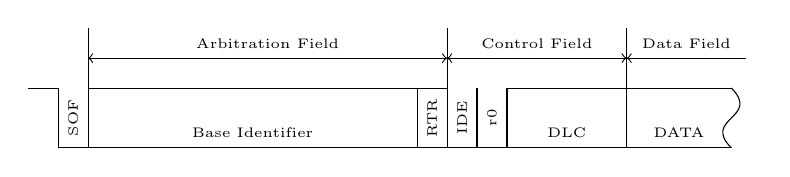
\begin{tikzpicture}[scale=0.76]
	%SOF
	\draw (0,1) -- ++(0.5,0) -- ++(0,-1) -- ++(0.5,0) -- ++(0,1);
	\node[rotate=90] at (0.75,0.5) {\tiny SOF};
	%Base Identifier
	\draw (1,1) -- ++(5.5, 0);
	\draw (1,0) -- ++(5.5, 0) node[midway, above=0.25] {\tiny Base Identifier};
	\draw (6.5, 0) -- ++(0,1);
	%RTR
	\draw (6.5, 0) -- ++(0.5,0);
	\draw (6.5, 1) -- ++(0.5,0);
	\draw (7, 0) -- ++(0,1);
	\node[rotate=90] at (6.75,0.5) {\tiny RTR};
	%IDE
	\draw (7, 0) -- ++(0.5,0);
	\draw (7.5, 0) -- ++(0,1);
	\node[rotate=90] at (7.25,0.5) {\tiny IDE};
	%r0
	\draw (7.5, 0) -- ++(0.5,0);
	\draw (8, 0) -- ++(0,1);
	\node[rotate=90] at (7.75,0.5) {\tiny r0};
	%DLC
	\draw (8,1) -- ++(2,0);
	\draw (8,0) -- ++(2,0) node[midway, above=0.25] {\tiny DLC};
	\draw (10, 0) -- ++(0,1);
	%data
	\draw (10,1) -- ++(1.75,0);
	\draw (10,0) -- ++(1.75,0) node[midway, above=0.25] {\tiny DATA};
	\draw (11.75,0) .. controls (11.25,0.5) and (12.25,0.5) .. (11.75,1);

	%Arbitration
	\draw (1,1) -- ++(0,1);
	\draw (7,1) -- ++(0,1);
	\draw[<->] (1,1.5) -- (7,1.5) node[midway, above] {\tiny Arbitration Field};
	%Control
	\draw (10,1) -- ++(0,1);
	\draw[<->] (7,1.5) -- (10,1.5) node[midway, above] {\tiny Control Field};
	%Data
	\draw[<-] (10,1.5) -- (12,1.5) node[midway, above] {\tiny Data Field};

\end{tikzpicture}
\caption{CAN Base Frame}
\label{fig:can_std_frame}
\end{figure}